% Foliensatz: "AFu-Kurs nach DJ4UF" von DK0TU, Amateurfunkgruppe der TU Berlin
% Lizenz: CC BY-NC-SA 3.0 de (http://creativecommons.org/licenses/by-nc-sa/3.0/de/)
% Autoren: Sebastian Lange <dl7bst@dk0tu.de>
% Korrekturen: Lars Weiler <dc4lw@darc.de>

\documentclass[aspectratio=169]{beamer}

\usepackage[ngerman]{babel} % deutsche Worttrennung etc.
\usepackage[utf8]{inputenc} % UTF8 Text

\usepackage[super, comma, numbers, square, sort]{natbib}

\usepackage{hyperref}       % Hyperref Package für bessere Referenzen (todo)
\hypersetup{
	colorlinks=false,       %   false: boxed links; true: colored links
    %linkcolor=white,       %   color of internal links (change box color with linkbordercolor)
    citecolor=red,          %   color of links to bibliography
    filecolor=white,        %   color of file links
    urlcolor=blue           %   color of external links
}

\usepackage{multirow}
\usepackage{wasysym}  % Math Symbols like \permil
%\usepackage{colortbl}
%\usepackage{subscript}
%\usepackage{caption}
%\usepackage{setspace}
%\usepackage{xcolor}        % benutze CodeListe

% Footnote
%\usepackage{hanging}
%
%\setbeamertemplate{footnote}{%
%  \hangpara{2em}{1}%
%  \makebox[2em][l]{\insertfootnotemark}\footnotesize\insertfootnotetext\par%
%}


%\usepackage{pgf}
%\usepackage{tikz}
%\usetikzlibrary{arrows,automata}
%\usetikzlibrary{positioning}
%
%\tikzset{
%    state/.style={
%           rectangle,
%           rounded corners,
%           draw=black, very thick,
%           minimum height=2em,
%           minimum width=2pt,
%           inner sep=2pt,
%           text centered,
%           },
%}

%\usepackage{listings}
%\lstset{basicstyle=\small, numberstyle=\tiny, extendedchars=true, numbers=left, numbersep=5pt}
%\lstset{showtabs=false, showspaces=false, showstringspaces=false}
%%\lstset{backgroundcolor=\color{white!75!lightgray}, , frame=single}
%%\lstset{backgroundcolor=\color{white}}
%%\lstset{backgroundcolor=none}
%\lstset{keywordstyle=\color{blue!50!gray},  identifierstyle=\color{black}}
%\lstset{commentstyle=\color{green!50!gray}, stringstyle=\color{red!50!gray}}
%\lstset{language=C, fontadjust=true, tabsize=2, breaklines=true}
%\lstset{backgroundcolor=\color{white!75!lightgray}, caption=\lstname, frame=single}
%\lstset{emphstyle=\color{black}\fbox}
%
%% Keine "Listing:"-Caption
%\captionsetup{labelformat=empty,labelsep=none}
%
%% für mathematische Umgebungen
%\usepackage{amsmath,amsfonts,amssymb}
%
%\lstdefinestyle{Bash}{
%language=Bash,
%frame=single,
%rulecolor=\color{black},
%backgroundcolor=\color{gray!50},
%keywordstyle=\color{black},
%identifierstyle=,
%commentstyle=\color{black},
%stringstyle=\color{magenta!65!white},
%showstringspaces=false,
%basicstyle=\footnotesize\ttfamily\color{black},
%numbers=none,
%breaklines=true,
%captionpos=b
%}

%\usepackage{listings}
%
%\lstdefinestyle{basic}{
%    captionpos=t,%
%    basicstyle=\footnotesize\ttfamily,%
%    numberstyle=\tiny,%
%    numbers=left,%
%    stepnumber=1,%
%    frame=single,%
%    showspaces=false,%
%    showstringspaces=false,%
%    showtabs=false,%
%    %
%    keywordstyle=\color{blue},%
%    identifierstyle=,%
%    commentstyle=\color{gray},%
%    stringstyle=\color{magenta}%
%}



% fließende Boxen haben keinen Abstand
%\fboxsep0mm

% inkludiere Creative Commons Helper
%%%%%%%%%%%%%%%%%%%%%%%%%%%%%%%%%%%%%%%%%%%%%%%%%%%%%%%%%%%%%%%%
%% ccBeamer 0.1, 2007-07-02                                   %%
%% Written by Sebastian Pipping <webmaster@hartwork.org>      %%
%% ---------------------------------------------------------- %%
%% Licensed under Creative Commons Attribution-ShareAlike 3.0 %%
%% http://creativecommons.org/licenses/by-sa/3.0/             %%
%%%%%%%%%%%%%%%%%%%%%%%%%%%%%%%%%%%%%%%%%%%%%%%%%%%%%%%%%%%%%%%%


%% Images
\newcommand{\CcImageBy}[1]{%
	
\includegraphics[scale=#1]{texdata/creative_commons/cc_by_30.pdf}%
}
\newcommand{\CcImageCc}[1]{%
	
\includegraphics[scale=#1]{texdata/creative_commons/cc_cc_30.pdf}%
}
\newcommand{\CcImageDevNations}[1]{%
	
\includegraphics[scale=#1]{texdata/creative_commons/cc_dev_nations_30.pdf}%
}
\newcommand{\CcImageNc}[1]{%
	
\includegraphics[scale=#1]{texdata/creative_commons/cc_nc_30.pdf}%
}
\newcommand{\CcImageNd}[1]{%
	
\includegraphics[scale=#1]{texdata/creative_commons/cc_nd_30.pdf}%
}
\newcommand{\CcImagePd}[1]{%
	
\includegraphics[scale=#1]{texdata/creative_commons/cc_pd_30.pdf}%
}
\newcommand{\CcImageSa}[1]{%
	
\includegraphics[scale=#1]{texdata/creative_commons/cc_sa_30.pdf}%
}
\newcommand{\CcImageSampling}[1]{%
	
\includegraphics[scale=#1]{texdata/creative_commons/cc_sampling_30.pdf}%
}
\newcommand{\CcImageSamplingPlus}[1]{%
	
\includegraphics[scale=#1]{texdata/creative_commons/cc_sampling_plus_30.pdf}%
}


%% Groups
\newcommand{\CcGroupBy}[2]{% zoom, gap
	\CcImageCc{#1}\hspace*{#2}\CcImageBy{#1}%
}
\newcommand{\CcGroupByNc}[2]{% zoom, gap
	\CcImageCc{#1}\hspace*{#2}\CcImageBy{#1}\hspace*{#2}\CcImageNc{#1}%
}
\newcommand{\CcGroupByNcNd}[2]{% zoom, gap
	\CcImageCc{#1}\hspace*{#2}\CcImageBy{#1}\hspace*{#2}\CcImageNc{#1}\hspace*{#2}\CcImageNd{#1}%
}
\newcommand{\CcGroupByNcSa}[2]{% zoom, gap
	\CcImageCc{#1}\hspace*{#2}\CcImageBy{#1}\hspace*{#2}\CcImageNc{#1}\hspace*{#2}\CcImageSa{#1}%
}
\newcommand{\CcGroupByNd}[2]{% zoom, gap
	\CcImageCc{#1}\hspace*{#2}\CcImageBy{#1}\hspace*{#2}\CcImageNd{#1}%
}
\newcommand{\CcGroupBySa}[2]{% zoom, gap
	\CcImageCc{#1}\hspace*{#2}\CcImageBy{#1}\hspace*{#2}\CcImageSa{#1}%
}
\newcommand{\CcGroupDevNations}[2]{% zoom, gap
	\CcImageCc{#1}\hspace*{#2}\CcImageDevNations{#1}%
}
\newcommand{\CcGroupNcSampling}[2]{% zoom, gap
	\CcImageCc{#1}\hspace*{#2}\CcImageNc{#1}\hspace*{#2}\CcImageSampling{#1}%
}
\newcommand{\CcGroupPd}[1]{% zoom
	\CcImagePd{#1}%
}
\newcommand{\CcGroupSampling}[1]{% zoom
	\CcImageSampling{#1}%
}
\newcommand{\CcGroupSamplingPlus}[1]{% zoom
	\CcImageSamplingPlus{#1}%
}


%% Text
\newcommand{\CcLongnameBy}{Attribution}
\newcommand{\CcLongnameByNc}{Attribution-NonCommercial}
\newcommand{\CcLongnameByNcNd}{Attribution-NoDerivs}
\newcommand{\CcLongnameByNcSa}{Attribution-NonCommercial-ShareAlike}
\newcommand{\CcLongnameByNd}{Attribution-NoDerivs}
\newcommand{\CcLongnameBySa}{Attribution-ShareAlike}

\newcommand{\CcNote}[1]{% longname
	This work is licensed under the \textit{Creative Commons #1 3.0 License}.%
}


% generelles Thema auswählen
\usetheme{Goettingen} %Berlin spart ohne Sidebar allerdings angenehm Platz
% AnnArbor | Antibes | Bergen | Berkeley | Berlin | Boadilla | boxes | CambridgeUS | Copenhagen | Darmstadt | default | Dresden | Frankfurt | Goettingen | Hannover | Ilmenau | JuanLesPins | Luebeck | Madrid | Malmoe | Marburg | Montpellier | PaloAlto | Pittsburgh | Rochester | Singapore | Szeged | Warsaw

% Farben wählen
\usecolortheme{beetle}
% beaver | beetle | crane | default | dolphin | dove | fly | lily | orchid | rose | seagull | seahorse | sidebartab | structure | whale | wolverine

% Setze alle Farben auf Grau und Weiß
%\definecolor{craneorange}{RGB}{64,64,64}
%\definecolor{craneblue}{RGB}{255,255,255}

% Schriftart wählen
\usefonttheme{default}
% default | professionalfonts | serif | structurebold | structureitalicserif | structuresmallcapsserif

% Innere Themen(Kopf-, Fuß-, Sidebar usw)
%\useinnertheme{default}
\useinnertheme{circles}
% default | inmargin | rectangles | rounded | circles

% Äußere Themen (Anordnung der inneren, grenzen der Folien etc.)
\useoutertheme{infolines}
% default | infolines | miniframes | shadow | sidebar | smoothbars | smoothtree | split | tree

% Deaktiviere Navigations-Symbole ({} -> leer)
\setbeamertemplate{navigation symbols}{}
%\setbeamertemplate{navigation symbols}{\large \ifnum \insertframenumber <10 0\fi\insertframenumber/\inserttotalframenumber\vspace*{0.2ex}}

% Zeige ein Hintergrundbild
\setbeamertemplate{background canvas}{
        \hspace*{-2.0cm}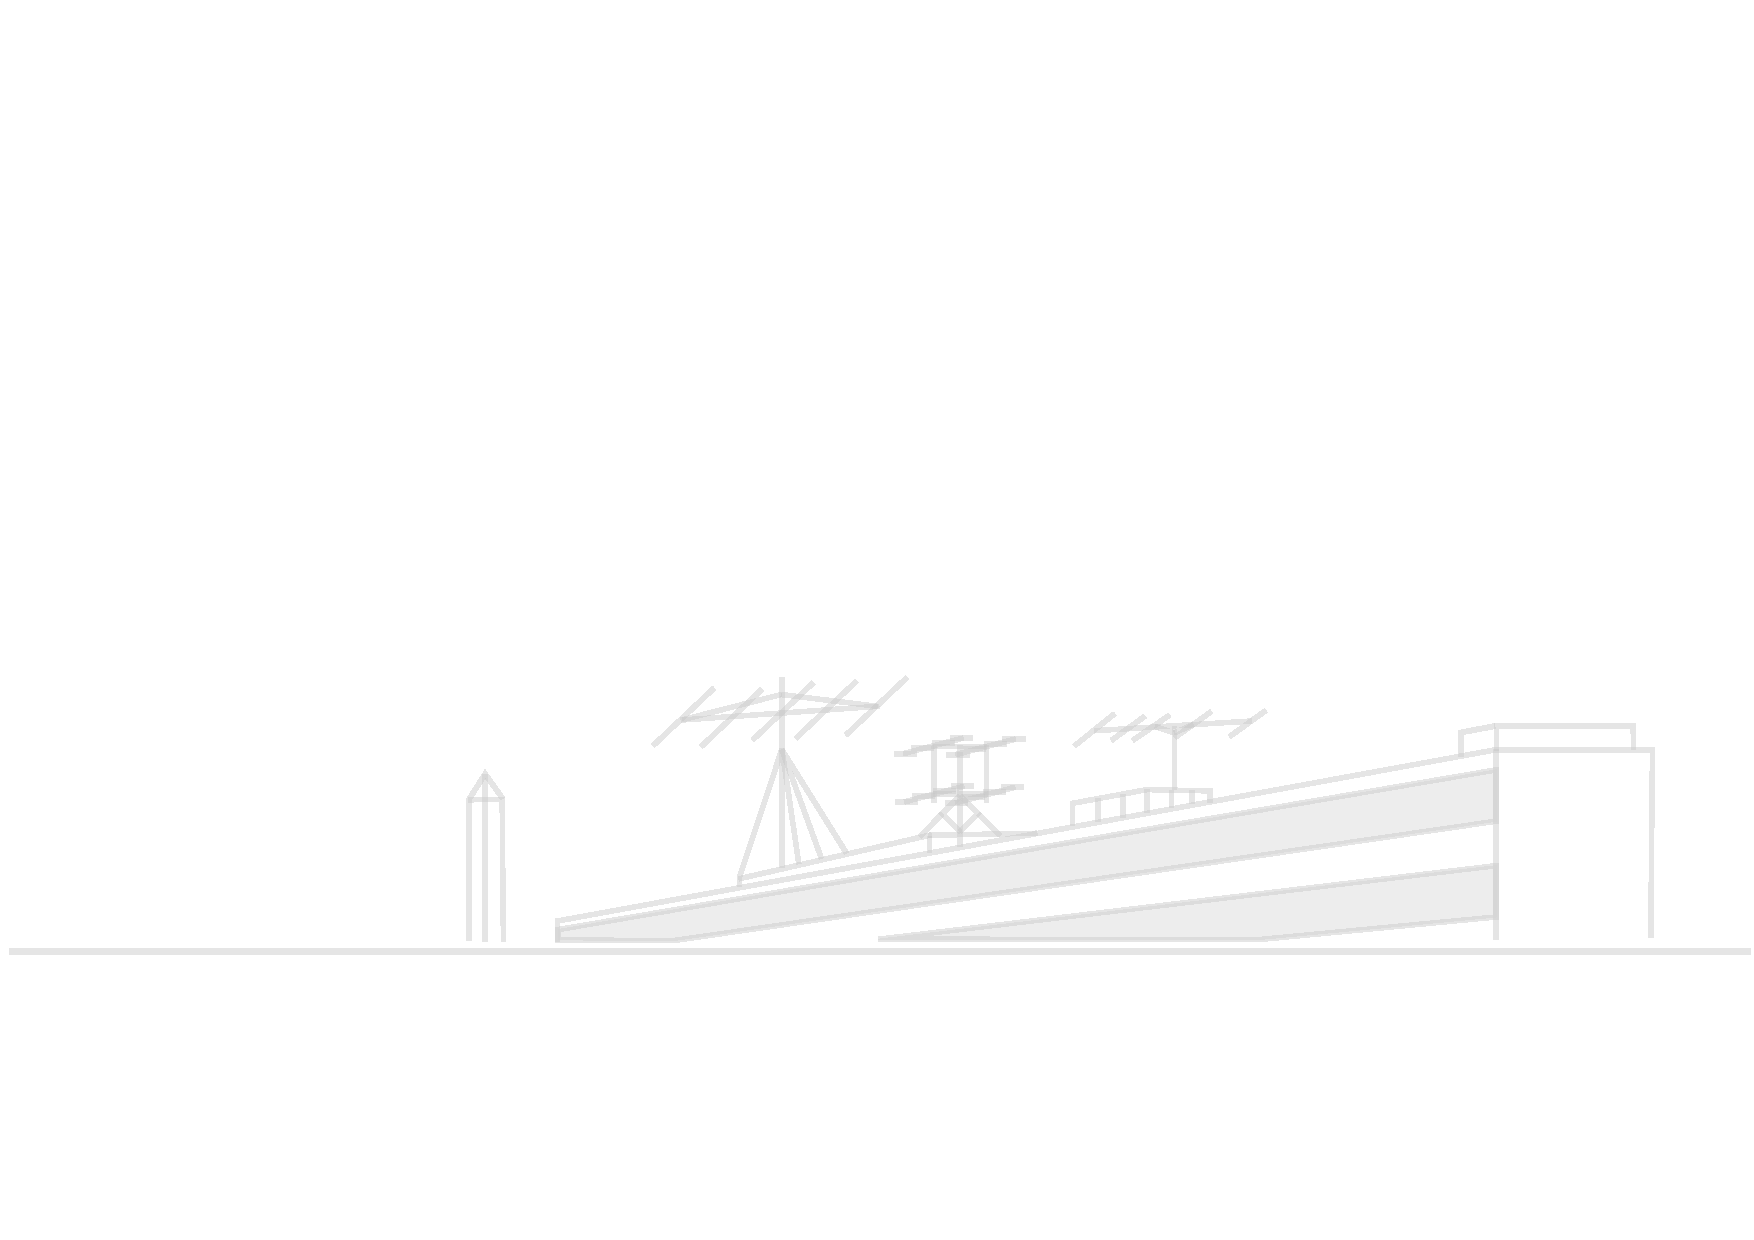
\includegraphics[width=17.8cm]{texdata/dk0tu_rooftop_background.pdf}
}

% Foliennummer einfügen
\setbeamertemplate{footline}[frame number]
%\setbeamertemplate{footline}{}

% Ändere das Zeichen vor jedem item
%\setbeamertemplate{itemize item}{\color{craneorange}$\blacktriangleright$}
%\setbeamertemplate{itemize subitem}{\color{craneorange}$\triangleright$}
%\setbeamertemplate{itemize subsubitem}{\color{craneorange}$\blacktriangleright$}

% Ändert die Blöcke 
\setbeamertemplate{blocks}[rounded][shadow=true]
% default | rounded [shadow=true|false]

%
% Eigene Kommandos
%

% Hack to get natbib and beamer working together. "The beamer user guide suggests
% that only the manual bibliography entry approach is supported"
% on some system it works out of the box, sometimes you need the hack :-(
% so check it --dl7bst
\ifdefined\newblock
    \relax
\else
    \newcommand{\newblock}{}
\fi

% \includedia command to generate png out of a dia file
% NEEDS installed dia and pdflatex option --shell-escape
\newcommand{\includedia}[1]{
    \immediate\write18{/usr/bin/dia #1.dia -e #1_diatmp.png -t png}
}

% RICHIG GROSSER FONT!
\newfont{\bigfont}{cmr10 at 144pt}
\newfont{\smallfont}{cmr10 at 8pt}

% Römische Ziffern
\makeatletter
\newcommand{\rmnum}[1]{\romannumeral #1}
\newcommand{\Rmnum}[1]{\expandafter\@slowromancap\romannumeral #1@}
\makeatother

% Schwarze Überschrift
%\setbeamercolor{frametitle}{fg=black}
%\setbeamercolor{title}{fg=black}

% Item- und Box-Farben
\definecolor{deepBlue}{HTML}{000066}
\setbeamercolor{itemize item}{fg=deepBlue}
\setbeamercolor{itemize subitem}{fg=deepBlue}
\setbeamercolor{description item}{fg=deepBlue}
\setbeamercolor{block title}{fg=deepBlue!100, bg=blue!15}
\setbeamercolor{block body}{fg=black, bg=blue!5}
\setbeamercolor{block title alerted}{fg=deepBlue, bg=red!75}
\setbeamercolor{block body alerted}{fg=black, bg=red!15}
\setbeamercolor*{block title example}{fg=blue!50, bg=blue!10}
\setbeamercolor*{block body example}{fg= blue, bg=blue!5}

%\setbeamercolor{section in head/foot}{parent=palette primary}
%\setbeamercolor{subsection in head/foot}{parent=palette secondary}
%\setbeamercolor{sidebar}{fg=darkblue,bg=yellow!90!orange}
%\setbeamercolor{title in sidebar}{fg=darkblue}
%\setbeamercolor{author in sidebar}{fg=darkblue}
%\setbeamercolor{section in sidebar}{fg=darkblue!10!black}
%\setbeamercolor{subsection in sidebar}{fg=darkblue!50!black}

% Titlepage Infos
\title{AFu-Kurs nach DJ4UF}
\author[DKØTU]{DKØTU\\ \footnotesize{Amateurfunkgruppe der TU Berlin}}
\institute[DKØTU]{\url{http://www.dk0tu.de} }

% PDF-Eigenschaften
\subject{DK0TU-Amateurfunkkurs nach DJ4UF}
\keywords{Amateurfunk Kurs HAM Radio Course CC-BY-NC-SA OpenSource TU Berlin DK0TU}

\subtitle{Technik Klasse A 01: \\
  Mathematische Grundkenntnisse \\[2em]}
\date{Stand 20.04.2017}
 \begin{document}

\begin{frame}
    \titlepage
    \vfill
    \begin{center}
        \ccbyncsaeu\\
        {\tiny This work is licensed under the \em{Creative Commons Attribution-NonCommercial-ShareAlike 3.0 License}.}\\[0.5ex]
         \tiny Amateurfunkgruppe der Technische Universität Berlin (AfuTUB), DKØTU
         %\includegraphics[scale=0.5]{img/DK0TU_Logo.pdf}
    \end{center}
\end{frame}

\section{Gliederung}
\begin{frame}
\frametitle{Gliederung}
\begin{itemize}
\item \textbf{Quiz}
\item \textbf{Dezibel}
  \begin{columns}[c]
    \column[c]{.8\textwidth}
\begin{itemize}
\item Leistungsgrößen
\item Feldgrößen
\item Leistungspegel
\item Spannungspegel
\item S-Stufen
\end{itemize}
\end{columns}
\end{itemize}
\end{frame}
\section{Einleitung}

\begin{frame}
  \frametitle{Einleitung}

  Diese Lektion baut auf dem Kapitel ``Mathematische Grundlagen und Einheiten
  (E01)''\footnote{vgl. \emph{Curriculum Klasse E}\hyperlink{refs}{\cite{curr}}} auf.

  \begin{columns}[c]
    \column[c]{.5\textwidth}
    Was bisher geschah: \\[1em]
    \begin{itemize}
      \item SI-Basissystem
        \begin{itemize}
          \item abgeleitete Einheiten
        \end{itemize}
      \item Präfixe/Zehnerpotenzen
      \item Formeln umstellen
    \end{itemize}
    \column{.5\textwidth}
    \begin{center}
      \begin{figure}
        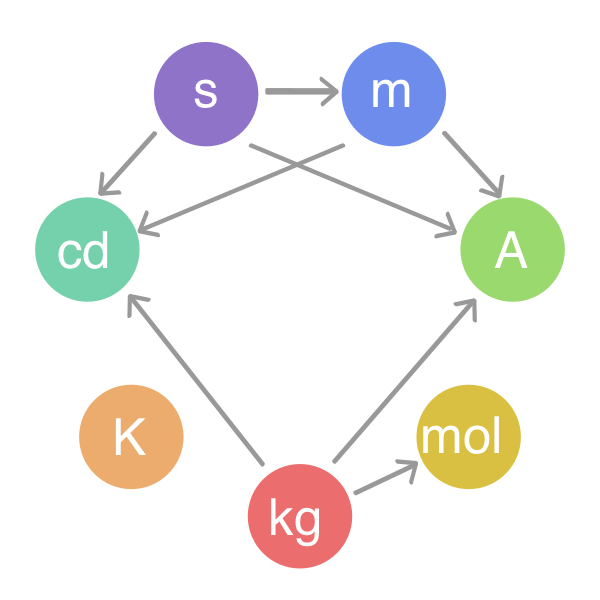
\includegraphics[width=.8\textwidth,height=.55\textheight,keepaspectratio]{e01/SI_base_unit.png}
        \attribcaption{SI Base Units}{Dono}{https://commons.wikimedia.org/wiki/File:SI_base_unit.svg}{\ccbysa}
      \end{figure}
    \end{center}
  \end{columns}

\end{frame}

\begin{frame}
  \frametitle{Einleitung / Unterschiede E und A}

  Was kommt dazu? \\[1em]

  \begin{itemize}
    \item im Prinzip: nichts
    \item jedoch tieferes Verständnis der Zusammenhänge und damit der
      Herangehensweise an den Rechenweg benötigt
    \item mathematische Grundlagen sollten ein sicheres Werkzeug sein
  \end{itemize}

\end{frame}

\begin{frame}
  \frametitle{Einleitung / Unterschiede E und A (vereinfacht!)}

  \vspace{1em}
  Klasse E:

  \begin{itemize}
    \item Formel finden
    \item Werte einsetzen
    \item lösen
  \end{itemize}

  \pause

  Klasse A:

  \begin{itemize}
    \item Zusammenhänge erkennen
    \item Formel(n) finden
    \item ggf. ineinander einsetzen oder mit Werten Teillösungen errechnen
    \item lösen
  \end{itemize}

  \pause

  \begin{center}\Large \emph{Don't Panic!}\end{center}

\end{frame}

\begin{frame}
  \frametitle{Einleitung / Reminder}

  Für die Prüfung bekommt man wie bei Klasse E die
  \textbf{Formelsammlung}\hyperlink{refs}{\cite{mat}} aus dem
  Anhang\footnote{S.131-138 (PDF-Seiten 133-140)} des Prüfungskataloges.\\[1em]

  Mitzubringen ist ein \textbf{nichtprogrammierbarer Taschenrechner}. \\[3em]

  $\Rightarrow$ Beides sollte man auch während des Kurses nutzen!

\end{frame}

\section{Wiederholung}

\subsection{Auffrischungsquiz}

\begin{frame}
  \frametitle{Auffrischungssquiz}

  \begin{exampleblock}{
    \only<1-2>{Was ist das \emph{MKSA}- bzw. \emph{MKSA-KMC}-System?}
    \only<3-4>{Welche Bedeutung haben die sieben Größen?}
    \only<5-6>{Zahlenbasis der SI-Einheiten?}
    \only<7-8>{Wie kann man $1337 \mu V$ auf 0,0001 $V$ genau/gerundet besser ausdrücken?}
    \only<9-10>{Rund wieviel $daW$ sind $\pi 10^{-3} kW$?}
    \only<11-12>{In welchen Größenordnungen liegen $\%$, $\permil$ und $ppm$?}
    \only<13-14>{Formel $20 lg \cfrac{x_1}{x_2} = y$ nach $x_2$ umstellen und berechnen.\\
    Gegeben: $x_1 = 8$ und $y = 12$}
    \only<15-16>{Was wurde mit der letzten Formel berechnet?}
    \only<17-18>{Gibt es einen einfacheren Weg?}
    }
    \only<1>{\vspace{2em}}
    \only<2>{SI-Einheitensystem aus: Meter, Kilogramm, Sekunde, Ampere, Kelvin, Mol, Candela}
    \only<3>{\vspace{1em}}
    \only<4>{Länge, Masse, Zeit, Stromstärke, Temperatur, Stoffmenge, Lichtstärke}
    \only<5>{\vspace{1em}}
    \only<6>{10}
    \only<7>{\vspace{4em}}
    \only<8>{$1 \mu V= 10^{-6}V$, \\
    $0,0001V = 0,1mV = 0,1 \cdot 10^{-3}V$ \\[1em]
    $\Rightarrow 1337 \mu V \approx 1,3 mV$}
    \only<9>{\vspace{2em}}
    \only<10>{$3,1416 \cdot \cfrac{10^{-3} \cdot 10^3}{10^1}W \approx 0,31 daW$
    \tiny $\leftarrow (Deka = \cfrac{1}{Dezi})$}
    \only<11>{\vspace{4em}}
    \only<12>{$10^{-2} \rightarrow$ Prozent ($c$) \\
    $10^{-3} \rightarrow$ Promille ($m$) \\
    $10^{-6} \rightarrow$ parts per million ($\mu$)}
    \only<13>{\vspace{4em}}
    \only<14>{$lg\cfrac{8}{x_2} = \cfrac{12}{20}$ \\
    $\cfrac{8}{x_2} = 10^{0,6}$
    $\Rightarrow x_2 = \cfrac{8}{10^{0,6}} \approx \cfrac{8}{4}$}
    \only<15>{\vspace{2em}}
    \only<16>{Die Eingangs\textbf{feldgröße} eines Systems mit $8$ am Ausgang und einer Verstärkung von $12dB$}
    \only<17>{\vspace{1em}}
    \only<18>{$12dB = 6dB + 6dB \approx$ Faktor $2 \cdot 2 \Rightarrow \cfrac{8}{2 \cdot 2}$}
  \end{exampleblock}

\end{frame}

\subsection{Dezibel}

\begin{frame}
  \frametitle{Dezibel-Rechnung}

  \ldots wurde bereits im Kapitel \emph{E10}\footnote{Dezibel, Dämpfung, Kabel} und
  bezogen auf die S-Stufen im Kapitel \emph{BV13}\footnote{RST-System, UTC, Logbuch, QSL-Karte}
  behandelt (vgl. \emph{Curriculum Klasse E}\hyperlink{refs}{\cite{curr}}). \\[2em]

  Für die Klasse A braucht man das etwas öfter. Daher eine kleine
  Wiederholung.

\end{frame}

\begin{frame}
  \frametitle{Dezibel / Motivation}

  Das Bel ist einheitenlos. Es deutet nur auf eine ``Transformation'' in den
  dekadisch logarithmischen Bereich hin. Warum der Aufwand?

  \pause

  \begin{itemize}
    \item große Wertebereiche können schnell überblickt werden
    \item im Gegensatz zu $ln$ einfach in Zehnerpotenzen
      kopfrechenbar\footnote{überschlagsweise}
    \item Rechenregel: Multiplikationen werden zu einfachen
      Additionen\footnote{damit auch Divisionen zu Subtraktionen}, z.B.
      \begin{itemize}
        \item Aufaddieren von Teilen einer Funkanlage
        \item Zerlegung einer Verstärkung in seine Faktoren
      \end{itemize}
  \end{itemize}

\end{frame}

\subsubsection{Leistungsgrößen}

\begin{frame}
  \frametitle{Dezibel / Leistungsgrößen}

  Gewinn/Dämpfung:

  \begin{center}
    $g = 10 \cdot lg \cfrac{P_{out}}{P_{in}} [dB]$
  \end{center}

  \vspace{2em}

  Werte die man (für die Praxis) im Kopf haben sollte:

  \begin{center}
    \footnotesize
    \begin{tabular}{|r|r|}\hline
      \textbf{Leistungsfaktor} & \textbf{Dezibel} \\ \hline \hline
      2                       &  3               \\ \hline
      10                       & 10               \\ \hline
    \end{tabular}
  \end{center}

\end{frame}

\subsubsection{Feldgrößen}

\begin{frame}
  \frametitle{Dezibel / Feldgrößen}

  %todo math. Zusammenhang?

  Gewinn/Dämpfung:

  \begin{center}
    $g = 20 \cdot lg \cfrac{U_{out}}{U_{in}} [dB]$
  \end{center}

  \vspace{2em}

  Werte die man (für die Praxis) im Kopf haben sollte:

  \begin{center}
    \footnotesize
    \begin{tabular}{|r|r|}\hline
      \textbf{Spannungsfaktor} & \textbf{Dezibel} \\ \hline \hline
      2                       &  6               \\ \hline
      10                       & 20               \\ \hline
    \end{tabular}
  \end{center}

\end{frame}

\subsubsection{Leistungspegel}

\begin{frame}
  \frametitle{Dezibel / Leistungspegel}

  Meist benutzt:

  \begin{itemize}
    \item $dBm$ bezogen auf $1 mW$ an $P_{in}$
    \item $dBW$ bezogen auf $1 W$ an $P_{in}$
  \end{itemize}

  \begin{center}
    Warum?
  \end{center}

  \pause

  Gewinne und Verluste in einer Kette können ab TX direkt miteinander
  verrechnet werden.

\end{frame}

\begin{frame}
  \frametitle{Dezibel / Leistungspegel-Beispiel}

  %\includedia{a01/TX-Pfad}
  \begin{figure}
    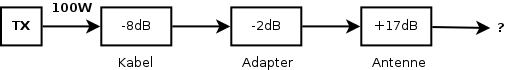
\includegraphics[width=1\textwidth]{a01/TX-Pfad}
    \caption{Weg beim Senden}
  \end{figure}

  \vspace{3em}

  \visible<2-4>{$20dBW - 8dB - 2dB + 17dB = 27dBW$ (in $W$?)\\}
  \visible<3-4>{$\Rightarrow$ Zerlege und Rechne: $30dBW - 3dB = $}
  \only<3>{$?$\footnote{genauer als naheliegendes $27dB \approx 20dB + 3dB + 3dB$}}
  \only<4>{$1000W \cdot \frac{1}{2}$}

\end{frame}

\subsubsection{Spannungspegel}

\begin{frame}
  \frametitle{Dezibel / Spannungspegel}

  Meist benutzt:

  \begin{itemize}
    \item $dB \mu V$ bezogen auf $1 \mu V$ an $U_{in}$
  \end{itemize}

  \begin{center}
    Warum?
  \end{center}

  \pause

  Gewinne und Verluste in einer Kette können ab \textbf{RX} direkt miteinander
  verrechnet werden.

\end{frame}

\subsubsection{S-Stufen}

\begin{frame}
  \frametitle{Dezibel / S-Stufen}

  Wurde ausfühlich in den Kapiteln \emph{E10}\footnote{Dezibel, Dämpfung,
  Kabel} und \emph{BV13}\footnote{RST-System, UTC, Logbuch, QSL-Karte}
  behandelt (siehe \emph{Curriculum Klasse E}\hyperlink{refs}{\cite{curr}})

  \begin{center}
    \begin{figure}
      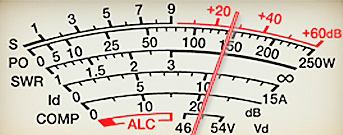
\includegraphics[width=0.4\textwidth,height=0.2\textheight,keepaspectratio]{e10/S-Meter.jpg}
      \attribcaption{S-Meter}{Cqdx}{https://commons.wikimedia.org/wiki/File:S-Meter.jpg}{\ccbysa}
    \end{figure}
  \end{center}

  %Erinnerungstest:

  \begin{exampleblock}{Was sind S-Stufen (Definition?) und ``Wie groß ist der
    Unterschied von S4 nach S7 in dB?'' (TA109)}
    \only<1>{\vspace{2em}}
    \only<2>{Definition $S9$: $5 \mu V$ (UKW) bzw. $50 \mu V$ (KW) an $50 \Omega$ \\[0.5em]
    $S4 .. S7 \equiv 3 \cdot 6dB = 18 dB$} %oder auch $\hat{=}$
  \end{exampleblock}

\end{frame}

\renewcommand{\refname}{Referenzen}

\hypertarget{refs}{}
\textcolor{white}{} \\ %\vspace{} geht nicht
\Large Referenzen/Links
\footnotesize

\begin{thebibliography}{}
    \setbeamertemplate{bibliography item}[online]
  \bibitem{darc} Moltrecht A 01: \\
    \url{https://www.darc.de/der-club/referate/ajw/lehrgang-ta/a01/}
  \bibitem{curr}  Curriculum Klasse E: \\
    \url{http://www.dk0tu.de/Kurse/AFu-Lizenz/Curriculum/Klasse_E/}
  \bibitem{mat}   Material und Dokumente für den Kurs: \\
    \url{http://www.dk0tu.de/Kurse/AFu-Lizenz#material}
\end{thebibliography}

% Hier könnte noch eine Kontaktfolie stehen

\end{document}

